% This is "sig-alternate.tex" V2.0 May 2012
% This file should be compiled with V2.5 of "sig-alternate.cls" May 2012
%
% This example file demonstrates the use of the 'sig-alternate.cls'
% V2.5 LaTeX2e document class file. It is for those submitting
% articles to ACM Conference Proceedings WHO DO NOT WISH TO
% STRICTLY ADHERE TO THE SIGS (PUBS-BOARD-ENDORSED) STYLE.
% The 'sig-alternate.cls' file will produce a similar-looking,
% albeit, 'tighter' paper resulting in, invariably, fewer pages.
%
% ----------------------------------------------------------------------------------------------------------------
% This .tex file (and associated .cls V2.5) produces:
%       1) The Permission Statement
%       2) The Conference (location) Info information
%       3) The Copyright Line with ACM data
%       4) NO page numbers
%
% as against the acm_proc_article-sp.cls file which
% DOES NOT produce 1) thru' 3) above.
%
% Using 'sig-alternate.cls' you have control, however, from within
% the source .tex file, over both the CopyrightYear
% (defaulted to 200X) and the ACM Copyright Data
% (defaulted to X-XXXXX-XX-X/XX/XX).
% e.g.
% \CopyrightYear{2007} will cause 2007 to appear in the copyright line.
% \crdata{0-12345-67-8/90/12} will cause 0-12345-67-8/90/12 to appear in the copyright line.
%
% ---------------------------------------------------------------------------------------------------------------
% This .tex source is an example which *does* use
% the .bib file (from which the .bbl file % is produced).
% REMEMBER HOWEVER: After having produced the .bbl file,
% and prior to final submission, you *NEED* to 'insert'
% your .bbl file into your source .tex file so as to provide
% ONE 'self-contained' source file.
%
% ================= IF YOU HAVE QUESTIONS =======================
% Questions regarding the SIGS styles, SIGS policies and
% procedures, Conferences etc. should be sent to
% Adrienne Griscti (griscti@acm.org)
%
% Technical questions _only_ to
% Gerald Murray (murray@hq.acm.org)
% ===============================================================
%
% For tracking purposes - this is V2.0 - May 2012

\documentclass{sig-alternate}

\begin{document}
%
% --- Author Metadata here ---
\conferenceinfo{WOODSTOCK}{'97 El Paso, Texas USA}
%\CopyrightYear{2007} % Allows default copyright year (20XX) to be over-ridden - IF NEED BE.
%\crdata{0-12345-67-8/90/01}  % Allows default copyright data (0-89791-88-6/97/05) to be over-ridden - IF NEED BE.
% --- End of Author Metadata ---

\title{Mobile Pickpocketing\titlenote{(Produces the permission block, and
copyright information). For use with
SIG-ALTERNATE.CLS. Supported by ACM.}}
\subtitle{Exfiltration of Sensitive Data through NFC-enabled Mobile Devices
\titlenote{A full version of this paper is available as
\textit{Author's Guide to Preparing ACM SIG Proceedings Using
\LaTeX$2_\epsilon$\ and BibTeX} at
\texttt{www.acm.org/eaddress.htm}}}
%
% You need the command \numberofauthors to handle the 'placement
% and alignment' of the authors beneath the title.
%
% For aesthetic reasons, we recommend 'three authors at a time'
% i.e. three 'name/affiliation blocks' be placed beneath the title.
%
% NOTE: You are NOT restricted in how many 'rows' of
% "name/affiliations" may appear. We just ask that you restrict
% the number of 'columns' to three.
%
% Because of the available 'opening page real-estate'
% we ask you to refrain from putting more than six authors
% (two rows with three columns) beneath the article title.
% More than six makes the first-page appear very cluttered indeed.
%
% Use the \alignauthor commands to handle the names
% and affiliations for an 'aesthetic maximum' of six authors.
% Add names, affiliations, addresses for
% the seventh etc. author(s) as the argument for the
% \additionalauthors command.
% These 'additional authors' will be output/set for you
% without further effort on your part as the last section in
% the body of your article BEFORE References or any Appendices.

%ANONYMIZED%%% \numberofauthors{8} %  in this sample file, there are a *total*
% of EIGHT authors. SIX appear on the 'first-page' (for formatting
% reasons) and the remaining two appear in the \additionalauthors section.
%
%ANONYMIZED%%% \author{
% You can go ahead and credit any number of authors here,
% e.g. one 'row of three' or two rows (consisting of one row of three
% and a second row of one, two or three).
%
% The command \alignauthor (no curly braces needed) should
% precede each author name, affiliation/snail-mail address and
% e-mail address. Additionally, tag each line of
% affiliation/address with \affaddr, and tag the
% e-mail address with \email.
%
% 1st. author
%ANONYMIZED%%% \alignauthor
%ANONYMIZED%%% Ben Trovato\titlenote{Dr.~Trovato insisted his name be first.}\\
       %ANONYMIZED%%% \affaddr{Institute for Clarity in Documentation}\\
       %ANONYMIZED%%% \affaddr{1932 Wallamaloo Lane}\\
       %ANONYMIZED%%% \affaddr{Wallamaloo, New Zealand}\\
       %ANONYMIZED%%% \email{trovato@corporation.com}
% There's nothing stopping you putting the seventh, eighth, etc.
% author on the opening page (as the 'third row') but we ask,
% for aesthetic reasons that you place these 'additional authors'
% in the \additional authors block, viz.
%ANONYMIZED%%% \additionalauthors{Additional authors: John Smith (The Th{\o}rv{\"a}ld Group,
%ANONYMIZED%%% email: {\texttt{jsmith@affiliation.org}}) and Julius P.~Kumquat
%ANONYMIZED%%% (The Kumquat Consortium, email: {\texttt{jpkumquat@consortium.net}}).}
%ANONYMIZED%%% \date{30 July 1999}
% Just remember to make sure that the TOTAL number of authors
% is the number that will appear on the first page PLUS the
% number that will appear in the \additionalauthors section.

\maketitle
\begin{abstract}

\end{abstract}

% A category with the (minimum) three required fields
\category{H.4}{Information Systems Applications}{Miscellaneous}
%A category including the fourth, optional field follows...

\terms{}

\keywords{}

\section{Introduction}
Near field communications (NFC) is a wireless communications technology most commonly built on the IEEE ISO 14443 Radio Frequency Identification (RFID) standard.  Although NFC was first standardized by the ISO/IEC in 2003 \cite{ecma-nfc-adoption}, until recently it has remained widely unused.  Now, NFC is becoming increasingly available to consumers, mainly through deployment in consumer mobile phones.  As NFC becomes more readily available to consumers, companies are considering ways to use the technology to provide new and enhanced services.

Foremost among those companies is Google.  In the past year and a half, no other major company has pushed as hard for rapid, widespread adoption and deployment of NFC hardware and software.  In early 2011, the company released a streamlined application programming interface to integrate newly-available NFC capabilities in mobile phone hardware with its Android platform \cite{nfcworld-nfc-additions-android-2.3.3}, and encouraged programmers to develop new and interesting NFC applications.  Their profit motive soon became clear.  By mid-year, Google announced Google Wallet \cite{google-blog-1}, an NFC-based payment system enabling mobile devices to function as payment cards at NFC-enabled retail terminals.  Google argues \cite{google-wallet-security-1} that a lockable, encrypted payment system using a secure element is safer than a standard credit card.  Whether or not these assertions are true remains to be seen.  While Google Wallet has suffered from high-profile security flaws \cite{esecurityplanet-google-wallet-hacked}, none of these resulted directly from its use of NFC.

Although its release of Google Wallet positions Google as a new and powerful force in consumer adoption of NFC technology, it is only one of the latest companies to enable the transfer of financial information through RF-enabled devices and tags \cite{smartcardaliance-more-visa-paywave}.  Credit Card companies have added RFID technology to their traditional magnetic stripe cards, giving two access vectors to the data stored within.  These RFID tags embedded in cards lack the necessary resources to offer the more sophisticated defenses of a smartphone.  As we will see, these so-called smart cards will divulge their data to any RFID reader that sends the correct sequence of commands.    

The susceptibility of such tags to RFID-enabled attack is not new \cite{picking-virtual-pockets} \cite{eavesdropping-attacks-hfrfid-tokens}; however, in the past these attacks were carried out with conspicuous, often custom-built RFID equipment.  The ability to read personal information via RFID on an inconspicuous consumer off-the-shelf device increases the stealthiness of an attack and eases a would-be attacker's access to the means of exploitation.  Security researchers analyzing this new variant of RFID attacks have dubbed it mobile pickpocketing.  

A mobile pickpocketing attack leverages the likely proximity between NFC-enabled phones and RFID-tagged cards to gather personally identifiable information (PII), thereby giving the attacker unauthorized access to the victim's sensitive data.  In mid-2011 ID Stronghold, the self-proclaimed ``\#1 manufacturer of RFID blocking wallets'' \cite{idstronghold-1} made a proof-of concept application:  a tic-tac-toe game equipped with trojan that would surreptitiously exfiltrate data to a remote server \cite{11alive-electronic-pickpocket-apps}.  Along with this distributed pickpocketing application, ID Stronghold ported the functionality of its custom-built RFID credit card reader into a mobile application.  Demonstrating similar research at Shmoocon 2012, Kristin Paget of the security consulting group Recursion demonstrated a similar attack \cite{forbes-1}.  Both sets of research were ostensibly done to promote the two companies' RFID-blocking card cases and wallets.  

In addition to mobile applications that can view credit card information \cite{idstronghold-1}, other mobile applications expose transit card data, such as trip information (departure location, arrival location, dates, times, etc.), when the card was refilled and how much was added, and the card's current balance \cite{farebot-1}.  The use of such an application could easily serve the needs of mobile pickpocket and legitimate user alike.  Although these sensational attacks seem viable, little record exists of any exploits actually occurring in the wild.  Yet as NFC capabilities become a standard feature on consumer mobile devices, attacks become easier to commit (the tools are more accessible) and more profitable (more victims possess the vulnerable technology).  Even so, companies that profit from NFC devices and companies that sell the security products that complement them cannot be trusted to give consumers a complete understanding of the potential risks of mobile pickpocketing.  Our research aims to fill that void.

This work discusses the process of building a proof-of-concept Android application that uses a consumer off-the-shelf mobile device's NFC features to read PII from both credit and transit cards.  We presume a reasonably skilled attacker could build such an application to exploit naive RFID communications, gaining PII from users within the application's proximity.  We developed the application for 2011 Samsung Google Nexus S phones and targeted PNC Visa payWave Virtual Wallet debit cards and Clipper transit cards.  We then tested the phone's ability to read data under various mobile pickpocketing-like circumstances.  We discuss our results and make recommendations to secure RFID PII transactions in the short and long term.  

\section{Building a Mobile Pickpocketing Application}
Inspired by ID Stronghold's Electronic Pickpocket application \cite{google-play-idstronghold}, we developed and tested an application of our own to better understand the capabilities and limits of mobile pickpocketing.  We worked on the application incrementally, beginning first with basic Android programming, and then building out RFID-reading capabilities until we could read data from Mifare Ultralight and Mifare Classic tags.  Then we moved on to the more complex task of reading and parsing credit and transit cards.    

Google's release of the Android NFC API greatly simplifies the process of discovering and reading NFC Data Exchange Format (NDEF) tags, but these libraries only provide full support for a subset of all the potential tag types that can be read using an NFC device. The Google API (as of version 2.3.3) provides documentation and code examples for Android applications reading data in Mifare Classic and Mifare Ultralight technologies.  Employing online documentation and code examples \cite{mifare-classic-detection-android} made these tag technologies fairly trivial to read.

These simple tag types make up only a small part of the NFC standard \cite{opennfc-1}.  The Android API allows a programmer to access any NFC-compatible tag technology, but doing so outside these fully-supported types is complicated \cite{android-developers-advanced-nfc}.  For NfcA, NfcB and IsoDep, the technologies used to read credit and transit cards, the Google API only provides a transceive method.  An application that accesses information from these types of tags must implement its own protocol stack on top of the built-in method.  To further complicate an RFID-reading programmer's task, each variant of RFID payment card has its own communications protocol.  For our proof-of-concept application, we focused on PNC Visa payWave cards.  After some initial trial and error, we discovered the cards use the NfcB subset of ISO 14443.  

After identifying the card's type, we set about extracting the card's data. Messages between the NFC device and the credit card can be exchanged through the use of Application Protocol Data Unit (APDU) commands. The ISO 7816-4 standard gave ready access to file system navigation commands, but eliciting valid responses (i.e. getting data) from the credit card required a knowledge of proprietary commands. This additional information is unique to the card vendor and, as far as we can tell, not publicly documented. Therefore, in order to identify the specific commands, we reverse engineered ID Stronghold's electronic pickpocket application \cite{idstronghold-1}. After analysis of the reversed applications, we identified credit card commands.  Applying this list of commands we began interrogating our PNC cards through a process of trial and error.  Once we were able to navigate the file system and extract the data in hexadecimal format, we saw that the data was unencrypted.  After that realization, exposing sensitive data was a simple matter of isolating the relevant hex output, converting it to human readable string data, and then returning the PII for display.     

A transit card requires more information to be stored on its NFC chip than a credit card, but the process of extracting information is similar.  To further facilitate transit card reaading, we analyzed FareBot, an open source application \cite{farebot-1} that reads a variety of transit cards.  Eric Butler, primary author of FareBot, noted that data in many transit cards is stored in the clear, an obvious privacy hazard.  The San Francisco Bay Area's Clipper Card, a card supported by FareBot, was one of these potentially data-exposing cards.  We obtained a Clipper card and set about extracting its information.  

The larger amount of data required for a transit card necessitates a different NFC technology.  Our research and Butler's code rely primarily on two NFC technologies: FeLiCa, which is developed and used by Sony (mainly in Asia), and Mifare DESFire. The Clipper Card and the ORCA (Seattle's transit card), are Mifare DESFire cards that use ISO 14443 A technology.  In order to interact with the Clipper Card, we programmed basic commands found in various tutorials for DESFire technology \cite{public-transport-card-exploits}.  With these commands, we were able to connect to the card, view the file structure, and receive records within those files.  The structure contains both data files and record files.  Although we did not have access to data files (the data files appear to be encrypted) the information presented in the unencrypted record files was sufficient to expose valuable PII.  Like the PNC payWave card, that information was returned from the card in hexadecimal format, and therefore not easily human-readable.  As a result, we followed the techniques Butler used in his code to parse and make sense of the information we found.  In our preliminary implementation, we were able to isolate the card's serial number, manufacturing information, card balance, and some available trip data.

\section{Attack Model}
Attacks using RFID are well documented \cite{picking-virtual-pockets} \cite{eavesdropping-attacks-hfrfid-tokens}, but until the advent of NFC, these attacks required conspicuous, custom-built readers, in many cases limiting the attacker's stealth.  While many of the devices implementing these attacks have the advantage of functioning at ranges far greater than NFC's ten centimeter limitation \cite{Kirschenbaum06howto}, a mobile pickpocket's weapon is an inconspicuous everyday object.  This is the attack model we assume:  a malicious user armed with only a consumer off-the-shelf, NFC-enabled mobile device running pickpocketing software.  We consider two vectors:  a physical attack, where the attacker uses his own device in close physical proximity to the victim's RFID card; and a distributed attack, where the attacker has surreptitiously placed his pickpocketing software on a user's device, thereby enabling remote exfiltration.  Let us first consider the former.  

As NFC phones continue to permeate the market, a physical attack becomes increasingly plausible.  While NFC is a rarity at present, the number of makes and models of mobile devices using the technology is increasing \cite{list-of-nfc-phones}.  The current cost of a Samsung Google Nexus S, the phone used in this research, is less than \$200 -- not a prohibitive investment for an aspiring data theif.  The cost of NFC phones will continue to decrease \cite{ds-nfc-enabling-technology}, further easing entry into the world of mobile pickpocketing.  While the Android platform does not provide direct access to more sophisticated NFC protocols, a savvy hacker has ample access to documentation on implementations of RFID-reading code posted on the Web.  As the technology becomes more pervasive, more applications will be built.  Better online, open Android RFID programming documentation will certainly follow.

A would-be pickpocket still has ample opportunity to perform a stealthy attack, despite the distance limitations of an NFC antenna.  Our physical attack model includes any attacker who can easily come within close proximity of a victim without raising suspicion.  Given the speed of a potential mobile pickpocketing attack, even a user giving up an RFID-enabled card for legitimate purposes is vulnerable to attack, even if the victim's card never leaves her sight.  For instance, a cashier might appear to use a phone to text friends while furtively stealing credit card information from an unsuspecting patron.  No greater stealth would be needed to use a phone to gain illegitimate access.  In a crowded mass transit system, it would be difficult to determine whether anyone holding a mobile device at waist level is trying to steal sensitive information.  Clearly the physical limitations of the attack are trivial.

Physical limitations can also be sidestepped entirely.  In recent years, data exfiltration trojans have been embedded into android programs, sending device data to foreign servers \cite{droiddreamlight}.  These trojans require additional application permissions above and beyond those required by any legitimate functions, enabling them to extract and send sensitive consumer data.  Adding stealth NFC-reading capabilities to such applications is entirely doable (as proven by ID Stronghold's game application).  True, the phone would have to be turned on and unlocked for an application to use its device's NFC, but even this barrier is easily surmountable.  The list of applications hosting these documented trojans includes active wallpaper and popular games \cite{venturebeat-malicious-wallpaper}, giving the attacker stealth NFC access to any tag within 10 cm while the malicious application is onscreen.  Given the frequent proximity of cell phones and wallets (purses, pockets, etc.), a successful exploit from an infected device seems all but inevitable: the attack only needs to work once.  

\section{Application Observations}
After finishing the credit card reading functionality of our Android application, we devised a set of heuristic tests to better understand the capabilities and limitations of a mobile pickpocketing attack from the perspective of a mobile user.  Here, we present our results and analysis from those tests followed by our recommended defenses.  

For application development, we used 2011 Samsung Google Nexus S phones running Android versions 2.3.6 and 4.0.4.  We tested our application using PNC Visa payWave debit cards issued in 2011 and a Clipper transit card issued in 2012.

The Android operating system itself imposes limitations on the use of NFC.  An Android mobile device will only conduct NFC interactions when the phone is powered on and unlocked.  The device must also have NFC enabled in its wireless 
\& network settings.  If all of the above are true, an Android phone is listening for NFC signals, and will react automatically when it senses a tag.  NFC connections are low-range and low-power, making them somewhat tenuous.  In its 2011 NFC API enhancements \cite{android-developers-nfc-basics}, Google presumed that a user might have multiple NFC-enabled applications on her mobile device.  To avoid interrupting a brittle NFC connection by requiring manual selection of an NFC application from a list of available options, the 2011 API update introduced streamlining features to direct-detected NFC information to the correct application automatically.  After clicking through a selection menu once, the application will then respond to NFC data in that same way for each subsequent interaction without further consultation of the user.  This enhancement to the user experience also enhances a clandestine attack.

Despite the exhortations of security companies selling RFID shields, a reasonable person might wonder:  if selecting an option from a popup menu is enough to undermine a legitimate NFC connection, how plausible is a real-world attack?  Armed with our card-reading Nexus S mobile devices, we decided to investigate.  We devised a set of heuristic tests based on the physical attack model, where an attacker attempts to access the victim's RFID information through her clothing and wallet and measured the results.  

Given the fragile nature of an NFC connection (we had surprisingly varied results trying to read credit cards, even under controlled circumstances), what sort of protection would a user's wallet and its contents provide?  We tested whether our pickpocketing application could read through a stack of cards, cards placed inside a wallet, and cards and wallet in the back pocket of a pair of jeans.  These results, too, were varied.

To test the protection offered by other cards, we began by placing a PNC payWave card on a non-metal surface.  We then stacked various other, non-RFID consumer cards on top, attempting to read the RFID tag on the bottom card with every new card added to the stack.  We used a variety of cards made from a variety of papers and plastics to simulate a typical consumer's wallet.  It took 15 cards before a Nexus S, placed on top of the stack, failed to read the RFID tag embedded in the credit card at the bottom of the stack.  We varied the cards and their order several times, but kept the amount of card material between the RFID chip and the reading device constant.  We measured the height of each varied stack with a digital caliper and found the cutoff range for data reading was an average of 9.94cm.  This defense only holds when the phone reads directly parallel to the tag, on top of the stack.  Reading the stack at an angle may still result in an effective read.  Clearly, other non-RFID cards do not provide reliable protection from a mobile pickpocket.  Interestingly, a stack with two PNC cards failed to register on the NFC reader.  However, pairing a PNC card with a Clipper card -- a Mifare DESFire transit card -- does not provide the same protection.  The PNC card is simply overpowered by the Clipper card, which is easily read.

Taking a stack of non-RFID cards placed around an RFID-enabled card and putting that stack into a wallet yields similar results.  10 cards inside a wallet still allows the Nexus S to read data when placed directly on top of the wallet containing the stack of cards inside, with the RFID-enabled card at the bottom.  Hence, it appears that a wallet in and of itself provides no more protection than a roughly equivalent width of cards.  As with the stack by itself, angle and position of the phone can undermine these crude defenses. Placing a wallet in the back pocket of a pair of jeans adds similarly negligible protection. We added the PNC RFID credit card to the contents of our wallets and found again that success of defense greatly depended on width of material between the RFID card and the Nexus S.  To further test defense by width of material, we measured the RFID-blocking properties of paper.  We found that it took an approximately 13.5cm stack of paper to block NFC connections.

While our experiments are admittedly informal, a clear conclusion can be drawn:  a wallet and its typical contents, placed inside clothing, offer no assurance of protection from a mobile pickpocket.  Even a victim who typically carries a large number of non-RFID cards is susceptible to attack.

We also tested the effects of a rubber Nexus S case \cite{ebay-epik-nexus-s-case}.  It provided no measurable defense, leaving a user open to a physical or distributed attack.  A special note:  we have seen mobile device cases \cite{ebay-fluffy-nexus-s-case} that store a user's cards precisely on top of a device's NFC antenna, placing a user's cards in an ideal position for a distributed attack.

\section{Defenses}
\subsection{Short-term}
While our simulations indicate that mobile pickpocketing is a viable attack, we also confirmed a few equally viable defenses.  We will discuss defenses easily accessible to a concerned user at present, as well as large-scale defenses that could be better protect all NFC-enabled mobile device users in the long term.

Our team did not test defensive card sleeves or wallets from either ID Stronghold or Recursion (Recursion's GuardBunny is not yet available to consumers).  It seemed unnecessary.  From our first readings of readable/writable Mifare tags through the parsing of the Mifare DESFire card, we observed that any metal in contact with an RFID tag would stop all NFC communications.  (As our research area was equipped with metal desks, we were reminded of this fact periodically throughout the duration of our research.)  This solution is easily extended to a consumer's wallet: tin foil is both inexpensive and effective.  Tin foil, even on the opposite side of either the the PNC payWave or Clipper card with respect to the reading mobile device, consistently kills NFC communications.  Limiting an attacker to consumer off-the-shelf mobile devices, the tin foil defense against mobile pickpocketing seems simple, cheap, and apt.

For the user who gets value from a card's RFID functionality, tin foil is a fine solution.  For a user who is uninterested in taking advantage of embedded RFID chips, destruction of the chip is a another simple, effective data defense that, when correctly implemented, eliminates any possible risk from an attack.  We will consider two methods of destruction.

Cooking the card in a microwave oven offers an effective way to disable an RFID chip, but the method is risky.  Microwaving the card for too long may destroy the non-RFID functionality of the card; leaving it in longer still increases the likelihood of a fire.  This is not the safest way to disable an RFID chip.

An equally effective, less flammable option is to crush the RFID chip inside the card.  While safer than the microwave option, it requires better aim.  The RFID chip can be tricky to find.  See Figure~\ref{fig:RFID_in_PNC_Card} and Figure~\ref{fig:RFID_chip_location} for details on the location of the PNC payWave's RFID chip.  Once the chip is identified, disabling the chip is simple: smashing it with a hammer should render the chip useless \cite{threat-analysis-of-rfid-passports}.  Once destroyed, the RFID chip will no longer communicate, thereby ensuring perfect data privacy.

	\begin{figure}%[H] %the [H] forces image placement
	  \centering
	  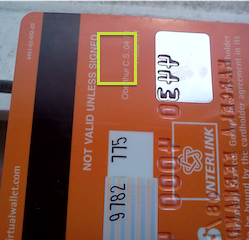
\includegraphics[width=0.3\textwidth]{images/RFID_in_PNC_Card.png}
	  \caption{Identifying an RFID chip}
	  \label{fig:RFID_in_PNC_Card}
	\end{figure}

	\begin{figure}%[H] %the [H] forces image placement
	  \centering
	  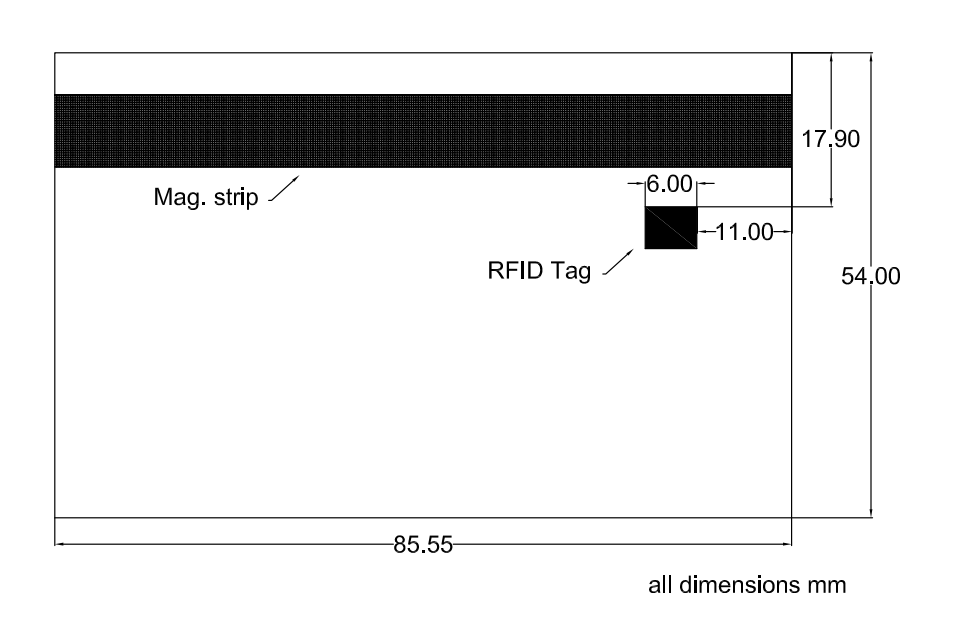
\includegraphics[width=0.4\textwidth]{images/RFID_chip_location.png}
	  \caption{Tag location: PNC payWave}
	  \label{fig:RFID_chip_location}
	\end{figure}

A warning for the user who would rather keep RFID tags intact: maintaining a safe 10 cm distance between RFID cards and devices is advisable, but as these objects naturally inhabit the same physical space, it would be unwise for a user to rely on this defense alone.  Assuming a user can continuously keep cards and readers separate, this defense only blocks a distributed attack from a phone that is physically in the user's control; as discussed above, an attacker able to read a fully-functioning RFID card at close range will still be able to do so, and need only do so once to compromise the victim's data.

Another word about distributed attacks: the normal, common sense caveats to Google Play application downloads should be of particular concern to the NFC-enabled user.  Be wary of the permissions an application requires.  If an application asks for more permissions than it needs, it could well be doing more than it says.  Google Play is still an unregulated market.  A user should consider downloading from a curated source.  The uninfected phone will not exfiltrate data.  

Each defense, regardless of its relative merits, postulates user awareness of the inherent risks of RFID-enabled cards.  For a user to decide on the most suitable defensive measures for mobile pickpocketing, she must first be aware of the technology she possesses and its configuration.  Approximately 100 million RFID-enabled cards are currently in circulation \cite{forbes-1}.  Through the course of our research, it seems many users are unaware that these devices are already a part of their everyday lives.  An ignorant user is a less wary user, and an easier target for a mobile pickpocket.

\subsection{Long-term}
Current RFID credit and transit cards require no authentication and implement no encryption of PII.  With no built-in defenses to overcome, mobile pickpockets who use applications to read sensitive information may not even qualify as hackers; they simply implement an open protocol \cite{bt-hacking-nfc-ccs}.  With payment and transit cards ready to divulge their data to any inquisitor with the correct sequence of commands, consumer data stored on these RFID cards is at continual risk of exfiltration.  As consumer NFC technology becomes more pervasive in mobile devices, that risk will only increase.

This level of exposure is surprising, considering that measures to secure RFID transactions of sensitive information are currently implemented in other domains.  Although RFID cards lack the power to perform the necessary functions for data security analogous to those seen in TLS communications for example, some RFID cards do provide better than non-existent security.  E-Passports, for instance, implement a PKI, facilitating secure encryption. They also link optical and RFID information, requiring information from both sources to access chip data, which renders the pickpocketing attacks described in this work moot \cite{security-privacy-epassports}.  The Navigo card used in Paris' mass transit system stores no PII; instead of a user or account number, each card is assigned an id number \cite{bt-hacking-nfc-ccs}.  Using encryption, authentication, and digital signatures, a point-of-service terminal can take the information stored on the card and use it to access sensitive information from the company through a secure channel between the company and the point of service.  This system prevents users from carrying their data around with them, minimizing the potential damage from a pickpocketing attack.  By not aiming to secure NFC itself, choosing instead to focus on securing the service that implements an NFC transaction, sensitive data is better protected, despite the limited resources of an RFID card.  

Perhaps U.S. credit card companies are getting wise to their card vulnerabilities.  As of January 2012, U.S. credit card companies are looking to not only further secure contactless cards, but ``...[move] toward a world beyond plastic...'' \cite{emv-upgrade}, better able to meet a variety of payment needs.  As mobile hardware moves toward widespread implementation in consumer mobile devices, working within the strict computational confines of RFID chips will become a far less attractive option. By comparison, industry and consumers alike will likely favor more robust device-based interactions over similar implementations using smart cards.  In this way, the mobile devices that make mobile pickpocketing such a dangerous problem are simultaneously the most attractive solution.     

The advantages of mobile devices over RFID cards are many.  With current technology, such devices already possess formidable computational power.  A typical smart phone has all the resources necessary to implement authentication, cryptography, and key management, allowing for functions like secure Internet browsing.  In Google Wallet, these functions are delegated to a so-called ``secure element,'' further cordoning off the application's cryptographic functions.  As in any modern operating system, mobile devices ship with native security features as well, including encryption, password protection, certificate storage, and locking screens.  Combining these standard features with those implemented inside an NFC payment application, such as Google Wallet \cite{google-wallet-security-1}, provides for multiple layers of authentication before data access is granted.  This level of depth and variety in security features makes mobile application-based payment an easy choice over RFID cards.  

While smart phones do offer greater security capabilities than smart cards, it's worth noting that these devices are not without their own security flaws.  Google Wallet in particular has had several known problems \cite{google-wallet-pin-cracked} \cite{smartphonechamp-second-major-flaw-google-wallet}.  Such flaws are to be expected; the technology is still maturing.  Better understanding current security shortcomings in NFC-enabled mobile devices will undoubtedly pave the way for future improvement.  Undoubtedly, as NFC applications endure further analysis from the security community, security for NFC payment and transit applications will advance.  

Some important solutions to better secure users against mobile pickpocketing are possible now.  Application market management appears highly effective \cite{electronista-mcafee-malware-surge}.  While the open Android market provides the more variety than its Apple counterpart, its unfettered freedom makes fertile ground for the rapid growth of malware.  Some attribute Apple's paucity of malicious iOS applications to its policy of strict capability limitations and application review.  Amazon recently opened a curated Android market \cite{amazon-android-appstore}; the impact of such curation on the security of Amazon-provided applications will be interesting to watch.  

A regulated marketplace would do well to identify always-on applications, such as live wallpaper, that use NFC functionality.  Devices implementing NFC for no clear application-related purpose should be blocked.

\section{Future Work}
Given the primary motivation for owning a mobile device is anytime, anywhere data connectivity, this study focused on researching and implementing a physical attack:  after achieving that goal, we assume that simply sending captured data would likely prove a trivial feature to implement.  Now that we have developed card-reading capability, the next logical step would be to embed that capability in a seemingly benign application (likely a live wallpaper or game).  We could use that legitimate portion of the application as a front for reading and stealthily exfiltrating RFID information gathered by the device on which our application is installed.  

Sending data over NFC in Android is becoming even easier.  In Android version 4.0, Google added Android Beam, \cite{ieee-beacon-mobileos-review} to its NFC library to further facilitate peer-to-peer NFC communications.  While the Google API suggests Beam will help users ``share contacts, web pages, and videos with other devices,'' \cite{android-developers-beam} any further encouragement of NFC data transfer can also serve a mobile pickpocket.  Could a malicious program allow for piggybacking unauthorized, sensitive NFC data along with transmissions from legitimate applications?  An in-depth look at those possibilities and their facilitation through Android Beam would be an interesting progression from this research.       

We found no balance data stored on the Visa payWave card; however, we have found the files where balance data is stored on the Clipper card.  As the Clipper is a Mifare DESFire card, with no known successful attacks \cite{farebot-1}, a next step in our research could involve implementing such an attack and assessing what defenses are in place.  Along with the current balance updated with each fare interaction, the card's files contain a card ID number.  Is the balance on the card associated with a balance record stored on the server side?  What other fraud prevention measures are in place?  What measures could be implemented?  As most mass transit systems are woefully underfunded, a widespread free-ride hack could prove extremely damaging to the public.

Some suggest replacing the credit card number stored on an RFID tag with a different identification number assigned by the card companies. While this certainly thwarts a mobile pickpocket from collecting a credit card number, it still leaves a victim's data compromised. An attacker could use an application such as ours to read this new ID from someone's credit card and subsequently perform a replay attack by emulating the tag for fraudulent payments at any one of many NFC-enabled payment kiosks.  Adding the ability to store and replay such information would diversify the threats of a future mobile pickpocketing application.  

\section{Conclusion}
The primary takeaways from our research into mobile pickpocketing are as follows:  despite any evidence or lack thereof of mobile pickpocketing in the wild, such attacks are a legitimate threat; users should be made aware of the technology involved and its risks, along with known defenses, so each can choose a course of action most appropriate to her needs; given the current climate of NFC implementation, the longer the public is ignorant, the more vulnerable it will become.


%
% The following two commands are all you need in the
% initial runs of your .tex file to
% produce the bibliography for the citations in your paper.
\bibliographystyle{abbrv}
\bibliography{adhawk-mobilepickpocketing}  % sigproc.bib is the name of the Bibliography in this case
% You must have a proper ".bib" file
%  and remember to run:
% latex bibtex latex latex
% to resolve all references
%
% ACM needs 'a single self-contained file'!
%
\]
\end{document}
